\section{Motivated Example}
\label{sec:motivation}

As described above, existing profilers cannot help identify some performance issues caused by the memory allocator. Let us use \texttt{threadtest} shown in Figure~\ref{fig:motivation} as an example. For this application, TcMalloc runs around $48\times$ slower than the default Linux allocator. We are using perf, gprof, and Coz for analyzing the performance of using the TcMalloc data.  The perf's result is shown in Figure~\ref{fig:mot1}, and gprof's result is shown as Figure~\ref{fig:mot3}. 

The perf tool reports that over 43\% time is actually spending inside \texttt{ld.so.2} library, which has nothing to do with the real example. For this application, TcMalloc actually introduces both active and passive false sharing issue, which is the major cause for this large slowdown. The gperf tool actually reports that 100\% time is spending inside the worker function, which also has no relation with the real issue. Similarly, Coz also cannot identify the issue that are caused by hardware contention~\cite{DBLP:conf/osdi/ZhouGMW18}. For this example, the first line of the code that can be improved by $XX$ is actually located in line $XX$ of \texttt{} file. That is also nothing related to the allocator.  

\begin{figure}[!ht]
\centering
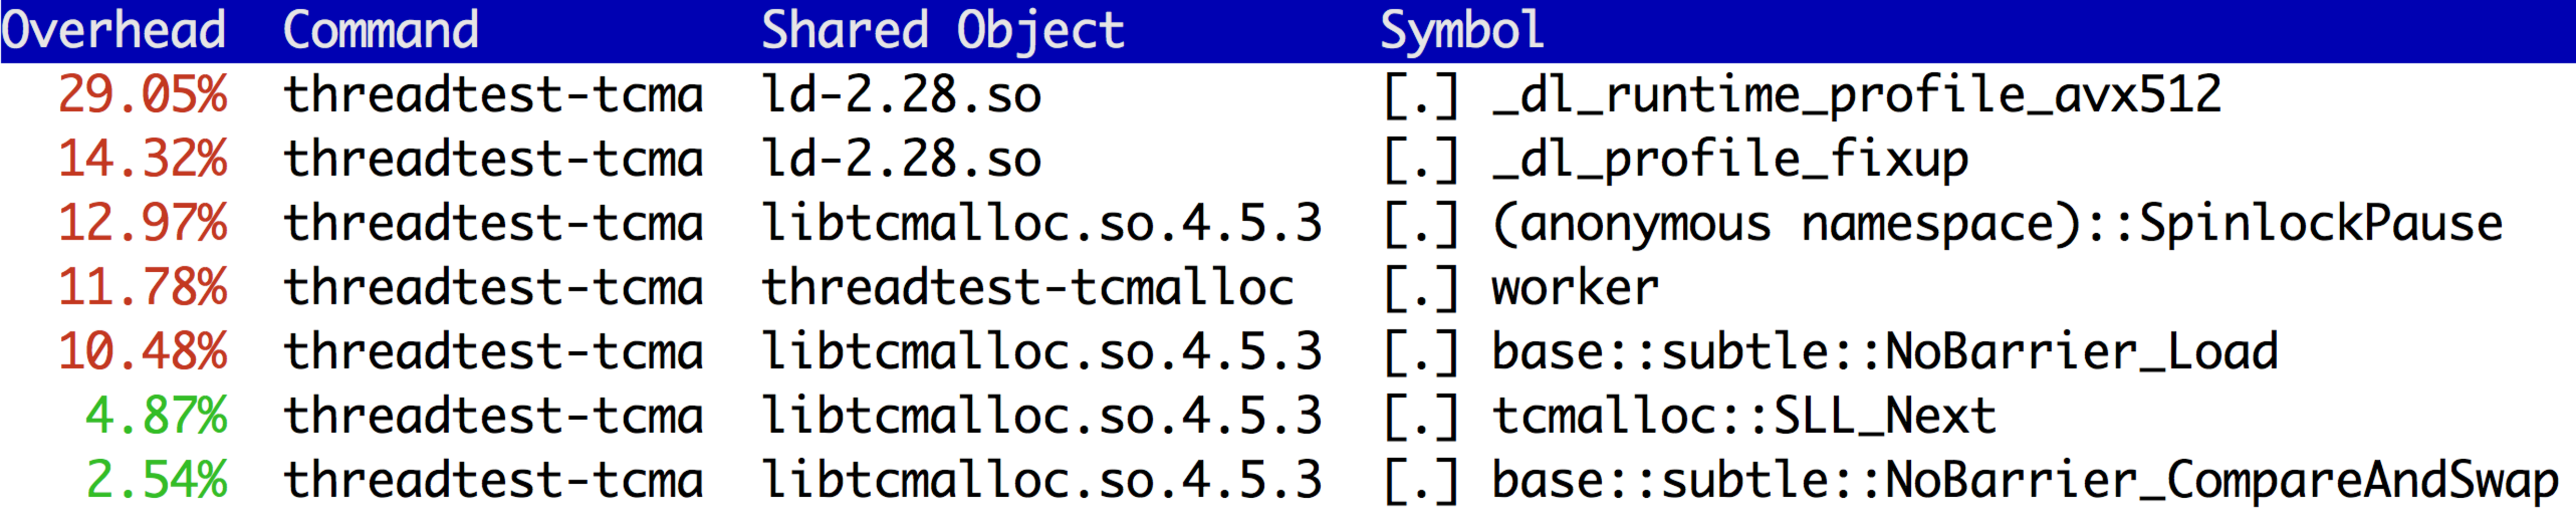
\includegraphics[width=\columnwidth]{figures/threadtest-tcmalloc}
\caption{Profiling result of perf, for \texttt{threadtest} with the TcMalloc allocator. \label{fig:mot1}}
\end{figure}

\begin{figure}[!ht]
\centering
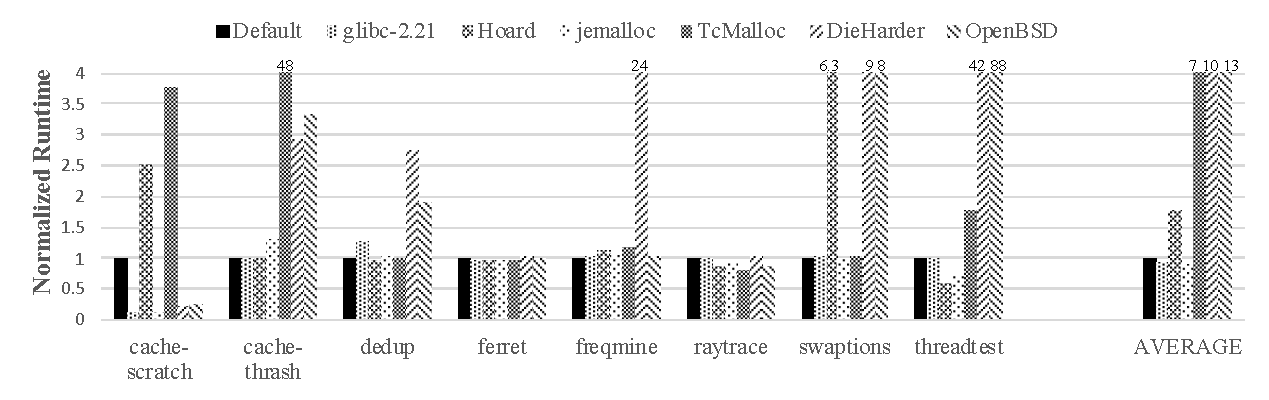
\includegraphics[width=\columnwidth]{figures/regular-performance}
\caption{Profiling result of gprof\label{fig:mot2}}
\end{figure}

In contrast, \MP{} reports this problem as passive false sharing issue, which is the real issue caused by the allocator. \MP{} reports a range of metrics for evaluating an allocator, such as memory overhead, and other issues. 

\section{Background and Overview}
\label{sec:background}

This section presents the background about memory allocators, and some important factors of allocators. Then the basic idea of \MP{} is presented. 

\subsection{Background of Allocator}

\label{sec:allocator}
Memory allocators are typically responsible for managing virtual memory inside the user space by satisfying memory requests from applications. Since the number of small objects is significantly larger than that of big objects, most allocators utilize different mechanisms to manage small and big objects. For big objects, allocators may obtain a block of memory from the OS directly during the allocation, and then return it to the OS upon the deallocation~\citep{Hoard}. For small objects, allocators may utilize freelists or bitmaps to track freed objects upon deallocations. In order to reduce external fragmentation and encourage memory utilization, memory blocks are managed by size classes, and every allocation will be rounded to its next largest size class.  

Based on the management of small objects, allocators can be further classified into multiple categories, such as sequential, BiBOP, and region-based allocators~\citep{DieHarder, Gay:1998:MME:277650.277748}. Region-based allocators are suitable for special situations in which all allocated objects within the same region are deallocated together~\citep{Gay:1998:MME:277650.277748}, which do not belong to the class of general-purpose allocators. Therefore, \MP{} mainly focuses on the other two categories of allocators, where most popular allocators belong to.

For sequential allocators, subsequent memory allocations are satisfied in a continuous memory block. Typically, a pointer is utilized to track the starting position of available space~\citep{Cling}. After an allocation, the pointer is bumped to the end of the current object, which is why this class is also known as ``bump-pointer allocators.'' For such allocators, objects with different sizes can be allocated continuously. Upon deallocation, a freed object is typically placed into the freelist of its size class. The size information of each object is typically physically placed just prior to the object. Such allocators include the default Linux allocator (originating from dlmalloc~\citep{dlmalloc}) and the Windows allocator~\citep{DieHarder}.  

BiBOP-style allocators, which stands for ''Big Bag of Pages''~\citep{hanson1980}, utilize one or multiple continuous pages that are treated as a ``bag'' used to hold objects of the same size class. The metadata of these heap objects, such as their size and availability information, are typically stored in a separate area. Thus, BiBOP-style allocators improve security and reliability by avoiding metadata corruption caused by buffer overflows. Many performance-oriented allocators, such as TcMalloc~\citep{tcmalloc}, \texttt{jemalloc}~\citep{jemalloc}, Hoard~\citep{Hoard}, Scalloc~\citep{Scalloc}, and most of secure allocators, such as OpenBSD~\citep{OpenBSD} and DieHarder~\citep{DieHarder}, belong to this category. BiBOP-style allocators may utilize freelists or bitmaps to manage the availability of objects. When using a bitmap, only a single bit is sufficient to track the availability of an object, which may introduce less memory overhead for the metadata, but possibly with a higher performance overhead due to the manipulation of the bitmap and the loss of temporal locality.  


\subsection{Important Metrics of Allocators}

\label{sec:factors}

Every memory allocator has its own design choices. However, they share many similar factors, such as performance, memory, scalability, and application-friendliness characteristics. This section will list important metrics for these factors, each of which will also be reported by \MP{}. 

\subsubsection{Performance}
\label{sec:performance}

The performance of using a memory allocator depends on two aspects, the performance overhead of its memory management operations, as well as its application-friendliness toward a specific application (as discussed in Section~\ref{sec: friendliness}). We will focus on the former item here. 

The performance overhead can be evaluated using the average number of instructions and the average runtime for each allocation and deallocation operation. The average data is more intuitive and understandable than the summary value alone. As described above, a memory allocator has different execution paths for different types of allocations and deallocations. Therefore, \MP{} further differentiates the type of memory operation during profiling, such as new or re-used allocations for small objects, deallocations for small objects, and allocations/deallocations for large objects. By doing this, \MP{} is able to identify an issue inside a particular execution path.
%\MP{} relies on a configuration file to obtain the threshold between small and big objects, and . 

In order to reveal a specific design issue, \MP{} further collects the averaged number of instructions, cache misses, and TLB misses for each operation, which are important factors for diagnosing performance issues. For instance, we use the number of cache misses inside DieHarder to diagnose its design issue for its memory deallocations. 
%a large number of instructions possibly indicates an inefficient design of an allocator. 

\subsubsection{Memory Consumption}
\label{sec:memoryconsumption}

Memory consumption is a serious concern across different platforms. Therefore, it is important to assess the memory consumption and wastage of a memory allocator. Sometimes, an allocator may waste more memory than that caused by memory leaks within an application. Based on our understanding, the memory consumption of an allocator may be attributed to multiple sources. First, it may originate from the metadata, such as the memory used to track the size or availability of every heap object. 

Second, it may be caused by internal fragmentation due to the particular set of size classes used (e.g. such as those used in a BiBOP-style allocator). As discussed above, memory allocators utilize multiple size classes to manage heap objects rather than using an exact size. The difference between the requested size and the size of the corresponding class represents its internal fragmentation, and this space cannot be utilized to satisfy other allocation requests. For instance, Hoard manages objects using power-of-two size classes~\citep{Hoard}, which thus may waste memory if the requested size is not an exact power-of-two. 
 
Third, memory allocator wastage may come from ``memory blowup.'' Memory blowup occurs due to the use of multiple heaps for the scalability purpose, where memory deallocations from one heap cannot be utilized to satisfy subsequent memory requests from another thread~\cite{Hoard}. 
%In order to solve this issue, Li et. al. employ heuristics to adjust the synchronization frequency dynamically~\cite{DBLP:conf/iwmm/LiLD19}. 
Since modern allocators typically utilize per-thread heaps or multiple arenas to reduce the contention overhead, memory blowup is a major source of memory consumption. However, it is challenging to actually quantify memory blowup, as further described in Section~\ref{sec:profilingmemory}.   

Fourth, memory consumption may come from external fragmentation. External fragmentation occurs when the total amount of the available memory is sufficient to satisfy a request but fails to do so due to the availability of only non-contiguous memory. External fragmentation is also related to the use of size classes, because allocators rarely or never perform object coalescing and splitting.
Usually it is impossible to change the size class for a few objects inside the bag, since BiBOP-style allocators typically use a single size for all objects in the entire bag. 
%That is, objects cannot be changed to other size classes, until all objects in the whole bag are freed. 
%This design may cause extensive external fragmentation overhead. 

 Lastly, some secure allocators may voluntarily skip certain objects in order to tolerate buffer overflows~\citep{DieHard, DieHarder, Guarder}. If a buffer overflow lands within these non-used objects, it will cause no harm to the application. However, it is extremely difficult to differentiate between explicit skipping and external fragmentation, with the effects of both ultimately being identical with regard to their impact on this type of memory overhead. 

Overall, for memory consumption, \MP{} individually reports the number and ratio of real memory usage, internal fragmentation, memory blowup, and other overhead. Other overhead includes external fragmentation, metadata overhead, and the sum of skipped objects. It is difficult for \MP{} to possess the precise information about the metadata and the sum of skipped objects. Therefore, \MP{} reports a summary for other memory overhead by subtracting the mentioned values from the total memory usage. For the total memory usage, \MP{} tracks memory-related system calls (e.g., such as \texttt{mmap} or \texttt{sbrk}). 
%Overall, \MP{} provides real memory usage of t
%\MP{} also reports real memory usage by tracking memory allocations and deallocations.  


\subsubsection{Scalability} 
\label{sec:scalability}

The scalability of an allocator can be affected by both hardware and software contention. Hardware contention is mostly related to cache or page contention, which is discussed in Section~\ref{sec: friendliness}. Software contention is the focus here, further including user space contention and kernel contention. 

\paragraph{User Space Contention} The user space contention of an allocator is typically caused by the use of locks inside memory management operations. Based on our observation, different allocators have significantly differing behaviors regarding lock usage. Some allocators, such as TcMalloc~\citep{tcmalloc} or jemalloc~\citep{jemalloc}, minimize the use of locks via per-thread cache. If an allocation can be satisfied from a per-thread cache, there is no need to acquire a lock. However, some allocators, such as Hoard~\citep{Hoard}, acquire at a lock for each allocation request, although using its per-thread heap.p. Some allocators, such as DieHarder and OpenBSD, utilize a central heap (and lock) for each size class, causing too much contention. 

%The average time for each lock acquisition indicates potential lock contention inside. The average time of each critical section helps expose whether the lock contention is due to the heavy workload inside the critical section or not. For instance, if the contention is high, but the average time inside the critical section is low, then this allocator should employ more fine-grained locks to distribute its overhead. In contrast, if the average time inside the critical section is high, then the allocator should possibly move some computation out of the critical section or simplify its management. 

To evaluate user space contention, \MP{} collects per acquisition data, per-operation data, per-lock data, and total information of locks. Per-acquisition data includes the runtime of each lock acquisition and the runtime of each critical section. For each operation, \MP{} reports the number of locks and the average runtime of each acquisition for different operations, such as new small allocations, re-used small allocations, small deallocations, and large allocations and deallocations. Further, \MP{} reports the total number of locks used inside the allocator, then reports the number of acquisitions, the contention rate, and the number of acquisitions for each operation for every suspicious lock that may have a contention issue. 
 
\paragraph{Kernel Space Contention} 
 An allocator may introduce kernel contention by invoking memory-related system calls frequently, such as \texttt{mmap}, \texttt{munmap}, \texttt{madvise}, and \texttt{mprotect}. These system calls may conflict with each other and with the page fault handler. By examining the source code of the Linux kernel, they all acquire a process-based lock (e.g. \texttt{mmap\_sem}) upon the entry of these system calls, causing kernel contention. Based on our evaluation, a version of the Linux allocator slows down an application by more than 20\%, due to extensive invocations of the \texttt{madvise} system call. Therefore, it is important to measure kernel space contention caused by a memory allocator. \MP{} proposes to utilize the average runtime of each system call to evaluate potential kernel contention, without the need to change the kernel source code.

For kernel contention, \MP{} reports the average time and the number of invocations for each memory-related system call. Since different operations (e.g., small versus large allocation) have different execution paths, \MP{} further reports the number for each particular operation. This differentiation helps identify an issue that may only appear in a particular operation pathway. 

\subsubsection{Application Friendliness}
\label{sec: friendliness}

Application friendliness indicates whether memory allocations are suited toward the access patterns of a particular application. Sometimes, application friendliness may have a larger impact on an application's performance than its memory management performance. For instance, TcMalloc typically has less memory management overhead than the default allocator, but runs around $48\times$ slower for \texttt{cache-thrash}. The major reason for this is that TcMalloc introduces both active and passive false-sharing~\cite{tcmallocsharing}. \MP{} reports multiple important metrics that evaluate application-friendliness.


The first parameter measured is the cache utilization rate. The cache utilization rate is the percentage of words that are currently holding actual objects. An allocator with a high cache utilization rate will cause less cache misses, benefiting the overall performance. Multiple causes may affect the cache utilization rate. First, some allocators (e.g., the Linux allocator) that prepend the metadata just prior to each object may reduce the cache utilization rate. Every cache load operation will load the metadata that is not referenced during normal memory access. 
 Second, a coarse-grained size class may also harm the cache utilization rate, due to internal fragmentation. Third, freed objects that are not reutilized in a timely manner may also cause a lower cache utilization rate. 

 %Similarly, if page utilization rate is low, it may cause high TLB misses and prohibitive memory consumption. \MP{} samples memory accesses, and checks the corresponding cache utilization rate and page utilization rate. Overall, \MP{} could report an average cache utilization rate and page utilization rate over all samples. 

The second parameter reported is the page utilization rate. The page utilization rate indicates the percentage of pages that are actively utilized for holding actual data. An allocator with a higher page utilization rate will introduce less page faults and less Translation Lookaside Buffer (TLB) misses. Lower page utilization rates can be caused by reasons similar to those that lower the cache utilization rate.  

The third parameter is the active/passive false sharing. False sharing indicates that multiple threads are concurrently accessing different words within the same cache line. Active false sharing is introduced upon the first allocations of objects, where an allocator cannot allocate continuous objects in the cache line to the same thread. Passive false sharing is introduced upon deallocations, where a freed object will be utilized by another thread, causing false sharing within the same cache line. 

The fourth parameter is the cache contention rate outside of the allocation. Cache misses can be caused by conflicting or falsely-shared misses. Upon cache misses, the data has to be loaded from the main memory, which is significantly slower than accessing the cache directly. 

Overall, \MP{} reports the cache utilization rate, page utilization rate, cache contention rate, and false sharing effect. For the false sharing effect, \MP{} not only reports the number of cache lines that have active and passive false sharing, but also reports the rate of conflicting accesses. The reported result also helps explain the performance slowdown issue. 
%employs the PMU hardware to collect these parameters. It employs the PMU-based sampling to sample memory accesses, and collects the data of cache and page utilization data upon sample events, as described in Section~\ref{sec:profilefriendliness}. \MP{} employs PMU to collect cache misses/page faults outside memory management.

\subsubsection{Summary of Important Metrics}

As described above, \MP{} reports many important metrics of an allocator, and is further shown in Table~\ref{table:metrics}. These metrics help answer whether an allocator is the culprit of a performance issue, and helps identify a particular design issue within the allocator. Table ~\ref{table:metrics} also provides collection techniques for specific metrics, which are further discussed in Section~\ref{sec:idea}. 

\begin{table}[h]
  \centering
  \caption{Important metrics and collection methods. Empty methods indicate that the metrics can be collected with simple counters.\label{table:metrics}}
  \footnotesize
 % \setlength{\tabcolsep}{1.0em}
\begin{tabular}{l | l | l}
\hline
Category & Important Metrics & Collection Techniques \\ \hline
\multirow{2}{*}{Performance} & {Alloc/Free runtime} & Timestamp\\ \cline{2-3}
& {Cache misses, page faults, TLB misses, instructions} & Performance Monitoring Units (PMU) \\ \hline
\multirow{4}{*}{Memory} & Internal fragmentation & \\ \cline{2-3}
	& Memory blowup &  \\ \cline{2-3}
& {Other overhead (e.g., external fragmentation)} &  \\ \cline{2-3}
& Real memory usage & \\ \hline
\multirow{2}{*}{Scalability} & \specialcell{User space contention: per-lock data} & Timestamp\\ \cline{2-3}
& {Kernel space contention: per-syscall data} &  Timestamp \\ \hline
\multirow{3}{*}{\specialcell{Application \\ Friendliness}} & Cache/page utilization rate & PMU  \\ \cline{2-3}
& False sharing effect &  PMU\\ \cline{2-3}
& Cache contention rate &  PMU \\ \hline
  \end{tabular}
\end{table}



